\documentclass[11pt]{article}

\usepackage{fancyhdr}
\usepackage{tikz}
\usepackage{subcaption}
\usepackage{xcolor}
\usepackage{geometry}

\geometry{tmargin=2cm,bmargin=2cm,lmargin=2cm,rmargin=2cm}

%theorem and definition environment
\usepackage{amsthm}

\usepackage{mathtools}

% From the assignment spec source *********************************
% Custom TikZ commands
\newcommand{\white}[3] {
  \foreach \x in {0, ..., #3} {
    \draw[fill=white] ({.5+#1},{\x*.1+.5+#2}) circle (0.42) node {#3};
  }
}
\newcommand{\black}[3] {
  \foreach \x in {0, ..., #3} {
    \draw[fill=white!70!black] ({.5+#1},{\x*.1+.5+#2}) circle (0.42) node {#3};
  }
}
\newcommand{\colorSquare}[3] {
  \draw[fill=#1] ({#2},{#3}) rectangle ({#2+1},{#3+1});
}

%******************************************************************

%defines a new amsthm environment in the 'definition' style
\theoremstyle{definition}
\newtheorem{definition}{Definition} %{environment name}{environment text}

%define equal symbol 
\def\defeq{\coloneqq}


%header and footer
\pagestyle{fancy}
\lhead{COMP30024 Artificial Intelligence}
\chead{}
\rhead{Assignment Part A}
\lfoot{}
\cfoot{\thepage}
\rfoot{}
\renewcommand{\headrulewidth}{0.4pt}

\begin{document}
    \begin{center}
        \textbf{\Large Assignment Part A}
        \medskip

        Rohan Hitchcock and Patrick Randell
    \end{center}
    Before reading the following, it is worth defining some terms that will be used throughout this report.
    \begin{definition} \label{defn:component}
        A \emph{component} is a subset of the black stacks on a board such that if one stack in the component explodes then all other stacks in the component will necessarily explode. 
    \end{definition}

    \begin{definition} \label{defn:goal}
        A \emph{goal set} (or \emph{goal}) is a subset of board positions in which a white token can explode in order to remove one or more components. For example, the set of positions surrounding a component could be a goal set.
    \end{definition}

    \section{Problem Formulation}\label{sec:problem-formulation}

    We approached this problem as an informed search problem on the space of valid board configurations, the goal of which is to arrive at a board configuration does not contain any black tokens via a sequence of valid white actions. Prior to beginning the search, we formulated the goal as follows. We first computed the set of components (Definition \ref{defn:component}) of the starting board configuration, and from this a set of goal sets (Definition \ref{defn:goal}) such that exploding a white token in all of the goal sets will remove all components -- and hence black tokens -- from the board. In the simplest case the goal sets are the set positions surrounding a component, however in some problems (such as in the second test case) goal sets must be formulated as intersection between positions surrounding two or more components. This decision was made based on the number of white tokens available. 

    We defined a state as a valid board configuration, which comprises of the position and height of all white and black stacks. Also included in the state are the remaining goal sets. Although it is possible to calculate these from the black stack data it is more efficient to transfer this data between states. A state is a goal state if and and only if its set of goal sets is empty, which is equivalent to a goal state containing no black stacks.

    The transitions from a state are given by the valid actions of white stacks. A valid white action is either moving some number of tokens from a stack to another position, or exploding a stack. In order to reduce the branching factor, we chose to only allow a white stack to do an explode action if it was in a goal state. 
    
    We defined the true cost of reaching a goal state from a state $S$ as the minimum number of white actions required to reach a goal state starting from $S$. This means each transition has cost one. 
    
    \section{Search Algorithm}\label{sec:search-algorithm}
    We decided to choose the A* search algorithm for this problem since it is complete and optimal (given an admissible heuristic). Experimentation showed that the memory use for A* was not prohibitive: the hardest problems required around 2000 nodes, which when considering the size of a node is in the order of 1Mb. Most problems do not require more than 100 nodes.

    \subsection{The heuristic}\label{subsec:heuristic}
    
    For some state, let $W$ be the set of white stacks and $G$ the set of goal sets. In a board with no other stacks, the minimum number of moves of a white stack $w \in W$ of height $n$ at position $(a, b)$ must take to reach position $(x, y)$ is 
    \[
        c(w, (x, y)) \defeq \left\lceil  \frac{| x - a |}{n} \right\rceil + \left\lceil  \frac{| y - b |}{n} \right\rceil.
    \]
    This is the $L^1$-norm dilated according to the movement speed of the stack. Since each goal set $g \in G$ is a set of board positions we define the distance of a goal to a white token to be
    \[
        c(w, g) \defeq \min _{(x, y) \in g} c(w, (x, y))
    \] 
    We defined the heuristic as the sum of the distance of each goal to its closest white token, plus the cost of exploding at each goal.
    \[
        h(W, G) \defeq \sum _{g \in G} \min _{w\in W} c(w, g) + |G|
    \]
    Note that the same white stack may be the closest stack to two or more different goals. While $h(W, G)$ would be a better approximation if each goal had a unique white token in the sum, computing this minimum proved to be more computationally expensive than the gains made by the improvement in the heuristic.

    A slight improvement can be made by observing that if $|W| < |G|$ then it is impossible to reach a goal state. This was incorporated into the heuristic like so:
    \[
        h'(W, C) \defeq \begin{cases}
            \infty & |W| < |G|\\
            h(W, C) & \textrm{otherwise}
        \end{cases}. 
    \]

    \subsection{Admissibility of the heuristic}\label{subsec:admissibility-of-the-heuristic}
    This heuristic is not admissible since it does not consider the potential advantage of stacking. For example in Figure \ref{fig:inadmissable-heuristic} the true cost is $3$ but our heuristic estimates 4.
    \begin{figure}[ht!]
        \centering
        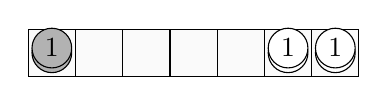
\begin{tikzpicture}[scale=0.6]
            \draw[fill=black!2!white] (0, 0) rectangle (7, 1);
            \draw[step=1] (0, 0) grid (7, 1);
            \black{0}{0}{1};
            \white{5}{0}{1};
            \white{6}{0}{1};
        \end{tikzpicture}
        \caption{}
        \label{fig:inadmissable-heuristic}
    \end{figure}
    This means that our implementation is not optimal. However it is worth noting that our implementation will still find the optimal solution in the situation of Figure \ref{fig:inadmissable-heuristic}. Despite the heuristic not being admissible, we believe that starting configurations for which our implementation finds a suboptimal solution are rare. The only examples of such configurations we have managed to find require a 10$\times$10 board.
    \section{Problem Features}
    The time and space complexity of A* is $\mathcal{O}(b^{d \cdot E(h)})$, where $b$ is the branching factor, $E(h) = \frac{|h - h^*|}{h*}$ is the error in the heuristic, and $d$ is the average depth of the solution.Let $n$ be the average stack size, $m$ the number of stacks and $g$ the number of goal sets. 
    
    The branching factor is $\mathcal{O}(m\cdot n!)$ since any number of tokens can be moved from any of the $m$ stacks. For most states $n \leq 3$, so taking $b = \mathcal{O}(m)$ is a reasonable estimate in the average case. 

    In a simple board configurations the depth of the solution $d$ is in the order of the length of the board and $E(h)$ is close to zero, however it is easy to come up with configurations where the depth and error is much is much higher. In these situations $E(h)$ roughly of the order of the length of the board. 
    
    One might think that increasing the number of goals can increase both $d$ and $E(h)$. While this is true to a point, when $g$ becomes too large both $d$ and $E(h)$ tend to drop because the board is dense with goal sets. Therefore $g$ does not play much of a roll except in pathological configurations. 

    This gives the complexity of our implementation to be $\mathcal{O}(m^k)$ where $k$ is somewhere between $0$ and $64$. The large range of $k$ suggests that the running time of our algorithm is far more dependent on the specific board configuration rather than the values of $n$, $m$ and $g$. This is supported by experimentation, where configurations with the same values of $n$, $m$ and $g$ can be designed to have very different running times by exploiting the strengths and weaknesses of the heuristic $h$.
\end{document}
